\documentclass[11pt, a4paper]{article}

% ---------- PACKAGES ----------
\usepackage[utf8]{inputenc}
\usepackage[T1]{fontenc}
\usepackage{amsmath, amssymb, amsthm, mathtools}
\usepackage{bm}
\usepackage{geometry}
\usepackage{graphicx}
\usepackage{booktabs}
\usepackage{longtable}
\usepackage{array}
\usepackage{hyperref}
\usepackage[table]{xcolor}
\usepackage{xcolor}
\usepackage{caption}
\usepackage{subcaption}
\usepackage{authblk}
\usepackage{listings}
\usepackage{pifont}  % for ✓ ✗ symbols
\usepackage{wasysym} % for ◐ ● symbols if needed
\usepackage{wasysym} % for ◐ ● symbols if needed
\usepackage{float}
\usepackage{tikz}
\usetikzlibrary{arrows.meta, positioning, shapes.geometric, fit, calc}

\geometry{margin=2.5cm}

% Shared TikZ styles for pipeline flowcharts
\tikzset{
  flowbox/.style={
    rectangle,
    rounded corners=2pt,
    draw=black!60,
    fill=blue!6,
    very thick,
    align=center,
    text width=3.0cm,
    minimum height=1.0cm,
    font=\small
  },
  flowdecision/.style={
    diamond,
    aspect=2.1,
    draw=black!60,
    fill=orange!12,
    very thick,
    align=center,
    text width=2.7cm,
    inner sep=1pt,
    font=\small
  },
  flowoutput/.style={
    rectangle,
    rounded corners=2pt,
    draw=black!60,
    fill=green!8,
    very thick,
    align=center,
    text width=3.1cm,
    minimum height=1.0cm,
    font=\small
  },
  flowarrow/.style={-{Latex[length=3mm]}, very thick, draw=black!70}
}

% Symbol shortcuts for survey tables
\newcommand{\full}{$\bullet$}        % full coverage (1.0)
\newcommand{\half}{$\circ\!\!\!\!\bullet$} % partial (0.5)  -- alternative below
\renewcommand{\half}{\textonehalf}
\newcommand{\none}{$\cdot$}          % none (0)
\newcommand{\fail}{\ding{55}}        % ✗

% ---------- THEOREM ENVIRONMENTS ----------
\theoremstyle{plain}
\newtheorem{theorem}{Theorem}[section]
\newtheorem{lemma}[theorem]{Lemma}
\newtheorem{proposition}[theorem]{Proposition}
\newtheorem{corollary}[theorem]{Corollary}
\theoremstyle{definition}
\newtheorem{definition}[theorem]{Definition}
\newtheorem{assumption}[theorem]{Assumption}
\newtheorem{remark}[theorem]{Remark}

% ---------- MATH SHORTCUTS ----------
\newcommand{\R}{\mathbb{R}}
\newcommand{\N}{\mathcal{N}}
\newcommand{\E}{\mathbb{E}}
\newcommand{\bx}{\mathbf{x}}
\newcommand{\given}{\,|\,}
\DeclareMathOperator{\MAD}{MAD}

% ---------- TITLE ----------
\title{\textbf{From Raw Wearable Signals to an Analysis-Ready HRV Pipeline:\\
Dataset Characterization, Missingness Handling, Smoothing Methodology,\\
and Candidate Change-Point Detection Methods}}

\author[1]{Jatin Dangi}
\author[1]{Aarush Ram Anandh}
\affil[1]{Koita Centre for Digital Health (KCDH)}

\date{\today}

\begin{document}
\maketitle

% =============================================================================
\begin{abstract}
% =============================================================================
This manuscript documents the construction of an analysis-ready Heart Rate
Variability (HRV) pipeline built on multimodal wearable recordings supplied
by our study partner. We describe the dataset, characterize the HRV signal
across ten properties (H1--H10) that jointly inform every downstream
methodological choice, formalize a principled approach to missingness, and
develop a smoothing stage based on a structural particle smoother with
harmonic components. We additionally survey and motivate a set of candidate
change-point detection (CPD) methods that build on the smoothed signal. The
present paper concludes at the point of presenting and motivating these
candidate CPD methods; the implementation, experimentation, and downstream
evaluation of CPD are reserved for subsequent work.
\end{abstract}

\tableofcontents
\newpage

% =============================================================================
\section{Introduction}
% =============================================================================

This work documents the pipeline construction phase of an HRV-based
physiological monitoring study. The objective is not to make a clinical
prediction; rather, it is to produce an analysis-ready signal whose
properties are respected at every stage and whose downstream use for
change-point detection is well-motivated. Figure~\ref{fig:pipeline-overview}
provides a complete overview of the data pipeline, from the incoming
multimodal patient data through HRV processing (missingness handling,
smoothing, change-point detection, annotation) and the overlay and
combinatorics step that feeds the downstream machine learning model.

\begin{figure}[H]
\centering
\resizebox{0.98\textwidth}{!}{%
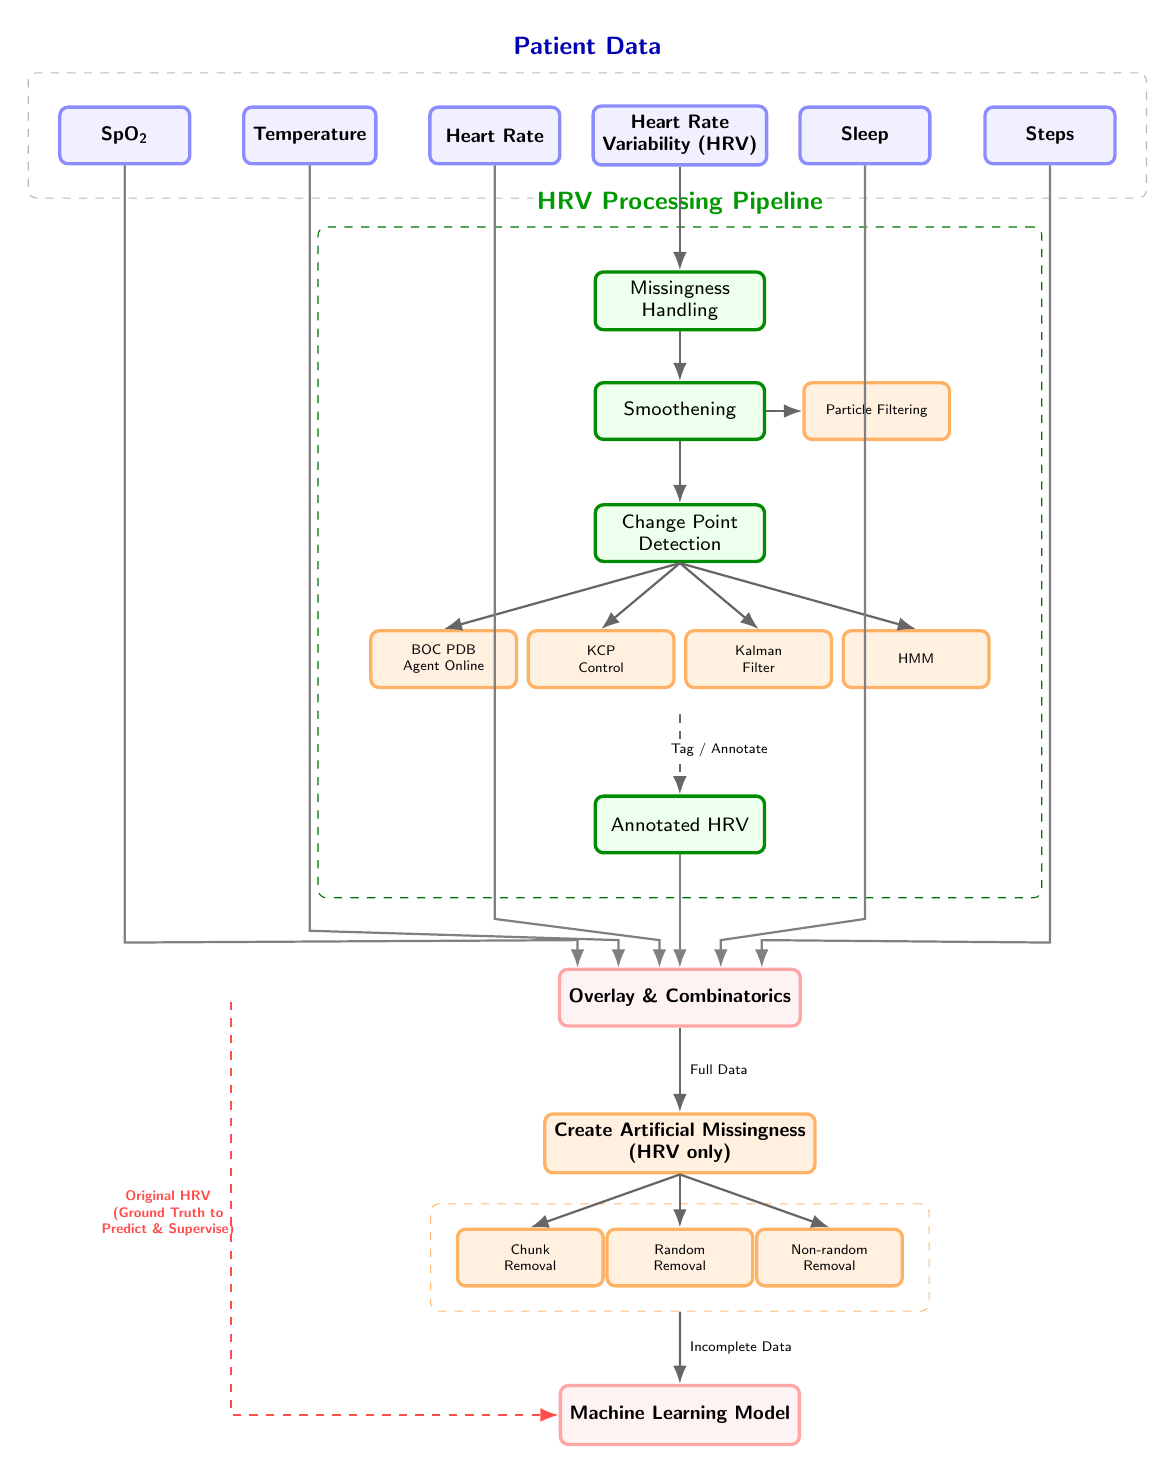
\begin{tikzpicture}[
  >=Latex,
  every node/.style={font=\sffamily\scriptsize},
  data/.style={rectangle, rounded corners=3pt, draw=blue!45, fill=blue!6,
    very thick, align=center, minimum width=1.65cm, minimum height=0.72cm},
  hrvstep/.style={rectangle, rounded corners=3pt, draw=green!55!black,
    fill=green!7, very thick, align=center, minimum width=2.15cm,
    minimum height=0.72cm},
  method/.style={rectangle, rounded corners=3pt, draw=orange!60,
    fill=orange!12, very thick, align=center, minimum width=1.85cm,
    minimum height=0.72cm, font=\sffamily\tiny},
  overlay/.style={rectangle, rounded corners=3pt, draw=red!35,
    fill=red!5, very thick, align=center, minimum width=2.85cm,
    minimum height=0.72cm, font=\sffamily\scriptsize\bfseries},
  miss/.style={rectangle, rounded corners=3pt, draw=orange!60,
    fill=orange!12, very thick, align=center, minimum width=3.25cm,
    minimum height=0.72cm, font=\sffamily\scriptsize\bfseries},
  ml/.style={rectangle, rounded corners=3pt, draw=red!35,
    fill=red!5, very thick, align=center, minimum width=2.95cm,
    minimum height=0.75cm, font=\sffamily\scriptsize\bfseries},
  pipearrow/.style={->, thick, draw=black!60},
  faintarrow/.style={->, thick, draw=black!50},
  redarrow/.style={->, thick, dashed, draw=red!70}
]
  % Top patient-data band
  \node[data, font=\sffamily\scriptsize\bfseries] (spo2) at (0,0) {SpO\textsubscript{2}};
  \node[data, font=\sffamily\scriptsize\bfseries] (temp) at (2.35,0) {Temperature};
  \node[data, font=\sffamily\scriptsize\bfseries] (hr) at (4.70,0) {Heart Rate};
  \node[data, font=\sffamily\scriptsize\bfseries] (hrv) at (7.05,0) {Heart Rate\\Variability (HRV)};
  \node[data, font=\sffamily\scriptsize\bfseries] (sleep) at (9.40,0) {Sleep};
  \node[data, font=\sffamily\scriptsize\bfseries] (steps) at (11.75,0) {Steps};
  \node[draw=black!28, dashed, rounded corners=3pt,
    fit=(spo2) (temp) (hr) (hrv) (sleep) (steps),
    inner xsep=0.38cm, inner ysep=0.40cm] (patientbox) {};
  \node[font=\sffamily\small\bfseries, text=blue!70!black]
    at ($(patientbox.north)+(0,0.34)$) {Patient Data};

  % HRV processing box
  \node[hrvstep] (missing) at (7.05,-2.10) {Missingness\\Handling};
  \node[hrvstep] (smooth) at (7.05,-3.50) {Smoothening};
  \node[method, minimum width=1.85cm] (pf) at (9.55,-3.50) {Particle Filtering};
  \node[hrvstep] (cpd) at (7.05,-5.05) {Change Point\\Detection};

  \node[method] (bocpd) at (4.05,-6.65) {BOC PDB\\Agent Online};
  \node[method] (kcp) at (6.05,-6.65) {KCP\\Control};
  \node[method] (kalman) at (8.05,-6.65) {Kalman\\Filter};
  \node[method] (hmm) at (10.05,-6.65) {HMM};

  \node[hrvstep] (annotated) at (7.05,-8.75) {Annotated HRV};
  \node[draw=green!45!black, dashed, rounded corners=3pt,
    fit=(missing) (smooth) (pf) (cpd) (bocpd) (kcp) (kalman) (hmm) (annotated),
    inner xsep=0.65cm, inner ysep=0.55cm] (hrvbox) {};
  \node[font=\sffamily\small\bfseries, text=green!60!black, fill=white, inner sep=1pt]
    at ($(hrvbox.north)+(0,0.30)$) {HRV Processing Pipeline};

  % Overlay and downstream data construction
  \node[overlay] (overlay) at (7.05,-10.95) {Overlay \& Combinatorics};
  \node[miss] (artificial) at (7.05,-12.80) {Create Artificial Missingness\\(HRV only)};
  \node[method] (chunk) at (5.15,-14.25) {Chunk\\Removal};
  \node[method] (random) at (7.05,-14.25) {Random\\Removal};
  \node[method] (nonrandom) at (8.95,-14.25) {Non-random\\Removal};
  \node[draw=orange!55, dashed, rounded corners=3pt,
    fit=(chunk) (random) (nonrandom),
    inner xsep=0.32cm, inner ysep=0.30cm] (missingbox) {};
  \node[ml] (mlmodel) at (7.05,-16.25) {Machine Learning Model};

  % Main HRV processing flow
  \draw[pipearrow] (hrv) -- (missing);
  \draw[pipearrow] (missing) -- (smooth);
  \draw[pipearrow] (smooth) -- (cpd);
  \draw[pipearrow] (smooth.east) -- (pf.west);
  \draw[pipearrow] (cpd.south) -- (bocpd.north);
  \draw[pipearrow] (cpd.south) -- (kcp.north);
  \draw[pipearrow] (cpd.south) -- (kalman.north);
  \draw[pipearrow] (cpd.south) -- (hmm.north);
  \draw[pipearrow, dashed] (7.05,-7.35) -- (annotated.north);
  \node[font=\sffamily\tiny, fill=white, inner sep=1pt] at (7.55,-7.80) {Tag / Annotate};

  % Overlay joins
  \coordinate (oinA) at ($(overlay.north)+(-1.30,0)$);
  \coordinate (oinB) at ($(overlay.north)+(-0.78,0)$);
  \coordinate (oinC) at ($(overlay.north)+(-0.26,0)$);
  \coordinate (oinD) at ($(overlay.north)+(0.52,0)$);
  \coordinate (oinE) at ($(overlay.north)+(1.04,0)$);
  \draw[faintarrow] (spo2.south) -- (0,-10.25) -- ($(oinA)+(0,0.35)$) -- (oinA);
  \draw[faintarrow] (temp.south) -- (2.35,-10.10) -- ($(oinB)+(0,0.35)$) -- (oinB);
  \draw[faintarrow] (hr.south) -- (4.70,-9.95) -- ($(oinC)+(0,0.35)$) -- (oinC);
  \draw[faintarrow] (annotated.south) -- ($(overlay.north)+(0,0)$);
  \draw[faintarrow] (sleep.south) -- (9.40,-9.95) -- ($(oinD)+(0,0.35)$) -- (oinD);
  \draw[faintarrow] (steps.south) -- (11.75,-10.25) -- ($(oinE)+(0,0.35)$) -- (oinE);

  % Artificial missingness and model-supervision flow
  \draw[pipearrow] (overlay) -- node[right, font=\sffamily\tiny] {Full Data} (artificial);
  \draw[pipearrow] (artificial.south) -- (chunk.north);
  \draw[pipearrow] (artificial.south) -- (random.north);
  \draw[pipearrow] (artificial.south) -- (nonrandom.north);
  \draw[pipearrow] (missingbox.south) -- node[right, font=\sffamily\tiny] {Incomplete Data} (mlmodel);

  \draw[redarrow] (1.35,-11.00) -- (1.35,-16.25) -- (mlmodel.west);
  \node[font=\sffamily\tiny\bfseries, text=red!70, align=center] at (0.55,-13.70)
    {Original HRV\\(Ground Truth to\\Predict \& Supervise)};
\end{tikzpicture}%
}
\caption{Complete data pipeline from incoming patient data through HRV
processing, change-point detection, overlay and combinatorics, and
downstream machine learning model.}
\label{fig:pipeline-overview}
\end{figure}

% =============================================================================
\section{Dataset and Signal Characteristics}
% =============================================================================

\subsection{Starting Point: Data Handover}

Our contribution begins after data acquisition. Raw multimodal recordings
provided by our study partner, GOQII including HRV (RR intervals), heart
rate, SpO\textsubscript{2}, skin temperature, step count, and sleep stages
were received in their device-native format. Before designing the pipeline,
we first examined the data frequency, quality, and related attributes
summarized in Table~\ref{tab:dataset-summary}. We then characterized the HRV
signal across ten properties that jointly informed every downstream
methodological choice, as presented in Table~\ref{tab:signal-characteristics}.

% --------------------- TABLE 1: DATASET SUMMARY ---------------------
\begin{table}[h!]
\centering
\caption{Dataset summary: signal modalities, trigger mechanism, cadence, and output format.}
\label{tab:dataset-summary}
\small
\begin{tabular}{p{2.2cm} p{2.6cm} p{1.8cm} p{1.8cm} p{1.6cm} p{2.6cm} p{1.0cm}}
\toprule
\textbf{Metrics} & \textbf{Trigger Mechanism} & \textbf{Data Nature} & \textbf{Frequency} & \textbf{Duration} & \textbf{Output Format} & \textbf{File Type} \\
\midrule
HRV & Automatic & Continuous & Every 10 minute & 10 min & Single HRV reading (e.g., 87) & .csv \\
Blood Pressure & User-Initiated (via button/app) & Discrete & On-demand & $\sim$60 seconds & Single BP reading (e.g., 120/80 mmHg) & .csv \\
Sleep & Auto-detected (movement \& HR analysis) & Continuous (captured) $\rightarrow$ Discrete & Throughout sleep duration & Full night & Sleep stages + total sleep duration & .csv \\
Heart Rate & Automatic / Continuous & Continuous & Every 5 minutes & Real-time sampling & BPM values across the day & .csv \\
ECG & User-Initiated (via button/app) & Discrete & On-demand & $\sim$44 seconds & ECG waveform with rhythm interpretation & .csv \\
SpO\textsubscript{2} & User-Initiated (via button/app) & Discrete & On-demand & 30--40 seconds & \% Saturation (e.g., 96\%) & .csv \\
Body Temperature & Automatic / Continuous & Continuous & Every 5--15 minutes & Real-time & Averaged skin/body temperature & .csv \\
Steps & Automatic via motion sensors & Continuous detection $\rightarrow$ Discrete & Real-time & Real-time & Cumulative daily step count & .csv \\
\bottomrule
\end{tabular}
\end{table}

\subsection{HRV Signal Characteristics (H1--H10)}

% --------------------- TABLE 2: SIGNAL CHARACTERISTICS ---------------------
\begin{table}[h!]
\centering
\caption{HRV signal characteristics (H1--H10) used as the design specification for downstream choices.}
\label{tab:signal-characteristics}
\small
\begin{tabular}{p{1.0cm} p{4.5cm} p{8.5cm}}
\toprule
\textbf{Code} & \textbf{Natural Language} & \textbf{Mathematical form} \\
\midrule
H1 & Bounded positive support & $X \in (0, X_{\max}]$; RR 200--1200~ms; RMSSD $\geq 0$ \\
H2 & Bimodal distribution & $\geq 2$ modes; mixture of underlying processes (likely day vs night HRV) \\
H3 & 1/f spectrum, long memory & $S(f) \propto 1/f^{\beta}$; ACF decays as power law (slowly) \\
H4 & Non-stationary & $\mu(t)$, $\sigma^{2}(t)$, $S(f,t)$ all time-varying \\
H5 & Circadian rhythm & Deterministic $\sim$24h periodicity \\
H6 & Heavy-tailed contamination & Motion bursts + ectopic point outliers; non-Gaussian noise \\
H7 & Non-uniform sampling & Irregular $\Delta t$ between observations \\
H8 & Mixed missingness & Random (motion artifacts) + non-random (off-wrist, charging) \\
H9 & Online (causal) operation & Estimator at $t$ uses only past observations \\
H10 & Between-patient variability & $\sigma^{2}_{\text{between}} \gg \sigma^{2}_{\text{within}}$; baselines vary widely across patients \\
\bottomrule
\end{tabular}
\end{table}

These ten characteristics are the design specification. Every subsequent
choice in this paper about what to discard, how to smooth, how to construct
ground truth, which change-point detectors to consider was guided by these
characteristics. Rather than imposing assumptions that simplify the signal,
our approach was designed to respect and preserve the intrinsic properties
of the data throughout the analysis pipeline.

% =============================================================================
\section{Data Handling and Preprocessing}
% =============================================================================

\subsection{Per-Patient Ingestion and HRV Isolation}

Data were received on a per-patient basis. We isolated the HRV channel for
cleaning and smoothing while leaving every other modality (steps,
SpO\textsubscript{2}, skin temperature, heart rate, sleep) untouched at this
stage; these covariates are re-introduced onto the common timeline only
after HRV has been cleaned and smoothed.

\subsection{Exploratory Data Analysis}

An exploratory analysis of the isolated HRV signal conducted at both the
per-patient level and across the pooled cohort surfaced the ten
characteristics enumerated in \S2.2. Plotting the value distributions
revealed a clear bimodal structure at both scales, with two distinct peaks
rather than a single central tendency (Figure~\ref{fig:raw-bimodal}). This
bimodality was treated as a structural property of the cohort and propagated
forward as a constraint on every downstream modeling choice.

\begin{figure}[h!]
\centering
\includegraphics[width=0.95\textwidth]{raw_bimodal.png}
\caption{Raw HRV signal (left) and value-frequency histogram (right) for a
representative patient, showing the bimodal distribution with two distinct
peaks rather than a single central tendency.}
\label{fig:raw-bimodal}
\end{figure}

\subsection{Characterizing Missingness}

The EDA also confirmed that missingness in the HRV channel was substantial
and of mixed type: both random (transient artifact, brief contact loss) and
non-random (device removal, charging, activity-coupled dropouts) gaps were
present in every patient's record. Because the two types carry different
physiological meanings, they could not be handled with a single blanket
imputation rule.

\subsection{The 180-Minute Chunking Rule}

HRV in this dataset arrives as a stream of roughly one reading every ten
minutes. A continuous stretch is one in which successive readings are
separated by approximately this cadence. When a gap appears for example,
readings at $t = 10, 20, 30, 100$, then nothing until $300$ the question is
whether the post-gap segment belongs to the same continuous record as the
pre-gap segment, or whether it should be treated as a fresh recording.

In consultation with domain experts, we consider a 180-minute threshold:
any inter-reading gap exceeding 180 minutes terminates the current segment,
and the next available reading begins a new segment. In the example above,
the readings at 10, 20, 30, and 100 are retained as one continuous chunk;
the gap from 100 to 300 (200 minutes) exceeds the threshold and triggers a
chunk boundary; readings from 300 onward (310, 320, 330, \ldots) form a new
continuous chunk.

\begin{figure}[H]
\centering
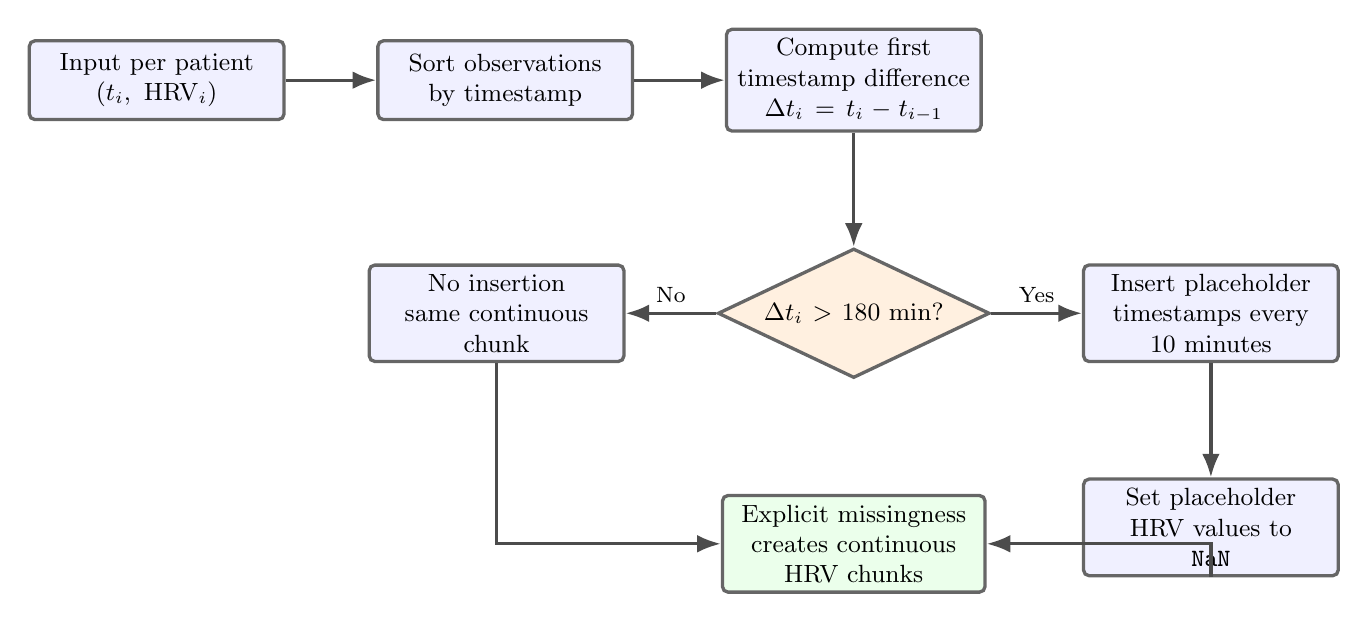
\begin{tikzpicture}[node distance=1.45cm and 1.15cm]
  \node[flowbox] (input) {Input per patient\\$(t_i,\ \mathrm{HRV}_i)$};
  \node[flowbox, right=of input] (sort) {Sort observations\\by timestamp};
  \node[flowbox, right=of sort] (diff) {Compute first\\timestamp difference\\$\Delta t_i=t_i-t_{i-1}$};
  \node[flowdecision, below=of diff] (decision) {$\Delta t_i > 180$ min?};
  \node[flowbox, left=of decision] (same) {No insertion\\same continuous\\chunk};
  \node[flowbox, right=of decision] (insert) {Insert placeholder\\timestamps every\\10 minutes};
  \node[flowbox, below=of insert] (nan) {Set placeholder\\HRV values to\\\texttt{NaN}};
  \node[flowoutput, below=of decision] (chunks) {Explicit missingness\\creates continuous\\HRV chunks};

  \draw[flowarrow] (input) -- (sort);
  \draw[flowarrow] (sort) -- (diff);
  \draw[flowarrow] (diff) -- (decision);
  \draw[flowarrow] (decision) -- node[above, font=\footnotesize] {No} (same);
  \draw[flowarrow] (decision) -- node[above, font=\footnotesize] {Yes} (insert);
  \draw[flowarrow] (insert) -- (nan);
  \draw[flowarrow] (same) |- (chunks);
  \draw[flowarrow] (nan) |- (chunks);
\end{tikzpicture}
\caption{Gap handling before smoothing. HRV observations are sorted by
timestamp, first differences between successive timestamps are computed, and
only gaps exceeding 180 minutes receive 10-minute \texttt{NaN} placeholder
rows. These placeholders expose missingness and naturally define continuous
chunks.}
\label{fig:gap-chunking-flowchart}
\end{figure}

The 180-minute cutoff was set by the domain experts on the basis of the
empirical distribution of inter-reading intervals locating the elbow points
in the gap-duration distribution (median, second, and third modes) combined
with physiological judgment about the timescale over which pre-gap autonomic
context can be considered informative for post-gap dynamics. Importantly,
data within retained chunks are not interpolated or back-filled; the
threshold operates only as a segmentation rule, not as an imputation rule,
preserving the missingness structure for the pseudo-ground-truth
construction in \S4.

% =============================================================================
\section{Handling Missingness}
% =============================================================================

Missingness in this dataset is not a nuisance to be removed; it is a
structural property of the signal that the pipeline must respect at every
stage.

\subsection{Why Standard Imputation Fails Here}

Mean imputation, forward-fill, and interpolation all assume that the gap is
a passive absence of measurement. In wearable HRV the gap is rarely passive:
the device was removed, the user was active, contact was poor, or the
signal was being lost precisely because something physiologically
interesting was happening. Replacing such gaps with smooth interpolants
would modify the raw data which leads to a possibility of incorrect
predictions.

\subsection{Where We Do and Do Not Impute}

We do not impute raw HRV for the purpose of producing a cleaner-looking
signal. Imputation enters the pipeline only inside the self-supervised
pseudo-ground-truth construction (\S4), where it serves a different
function: a model is trained to predict held-out values, and the prediction
error, not the imputed value, is the signal of interest.

% =============================================================================
\section{Smoothing}
% =============================================================================

\subsection{Why Smoothing in the First Place}

Several of the characteristics identified in \S2.2 heteroscedastic noise,
artifact contamination, and non-stationarity in particular guarantee that
any analysis run directly on raw HRV will be driven by noise rather than by
physiology. A smoothing stage that estimates the latent physiological state
under noise is therefore a structural requirement before any downstream
modeling can proceed.

\subsection{Cross-Disciplinary Survey and Scoring System}

Rather than default to a familiar smoother, we conducted a structured
survey of smoothing and state-estimation methods drawn from across fields
like statistics, signal processing, physics, control theory, econometrics,
and machine learning. Each method was scored against the ten HRV
characteristics (H1--H10) using a simple rubric: 1 point if the method
natively handles or makes assumptions consistent with the characteristic,
0.5 points if it can be modified to handle the characteristic with
techniques already documented in the literature, and 0 points otherwise.
The full survey appears as Table~\ref{tab:smoothing-survey} in
Appendix~\ref{app:smoothing-survey}.

\subsection{Selection of the Particle Filter}

The particle filter (sequential Monte Carlo, SMC) scored highest under this
rubric. It natively handles 7 of the 10 characteristics and can be modified
to handle the remaining 3 using extensions that are well established in the
literature. On this basis we selected the particle filter as the smoothing
backbone and proceeded to implement a modified version tailored to HRV; the
specific modifications are detailed in \S6.

Figure~\ref{fig:smoothing-results} shows the output of the structural
particle smoother on a representative patient: the raw HRV stream, the same
stream with $>$180-minute gap markers, the smoothed signal (level $+$
circadian) with its 95\% credible band, and the underlying trend (level
only, circadian removed).

\begin{figure}[h!]
\centering
\includegraphics[width=0.95\textwidth]{smoothing_results.png}
\caption{Structural particle smoother outputs on patient \texttt{0010}. Top
to bottom: raw HRV; raw with $>$180-minute gap markers; smoothed signal
(level $+$ circadian) with 95\% credible band; underlying trend (level
only, circadian removed).}
\label{fig:smoothing-results}
\end{figure}

% =============================================================================
\section{Structural Particle Smoother with Harmonic Components}
% =============================================================================

This section formalizes the particle smoother selected in \S5.3 as our
HRV smoothing backbone. The mathematical content below specifies the
state-space model, the observation model with missing-data handling, the
data-driven parameter estimation procedure, and the sequential Monte Carlo
forward filter and forward-filter backward-sampler used to produce smoothed
trajectories and credible intervals.

\subsection{Overview and Motivation}

This implementation extends the basic local-level-plus-slope particle
smoother to a full \emph{structural time series} model (Harvey, 1989).
Three components are superimposed to model HRV:

\begin{enumerate}
  \item A \textbf{local linear trend} $(\ell_t, s_t)$ capturing the slowly
    varying physiological baseline.
  \item A \textbf{daily harmonic} $(c_t^{(1)}, c_t^{*(1)})$ capturing
    circadian (24-hour) HRV rhythms.
  \item A \textbf{semi-daily harmonic} $(c_t^{(2)}, c_t^{*(2)})$ capturing
    the 12-hour ultradian rhythm (rest/activity alternation).
\end{enumerate}

The observation model uses a Student-$t$ likelihood (heavy tails, robust to
motion artefacts) and explicitly handles missing observations via a flat
likelihood, so the filter does not require pre-segmentation into continuous
chunks. Parameters are estimated from the data before filtering using a
robust median-absolute-deviation (MAD) procedure.

\subsection{State Vector and Initial Distribution}

\begin{definition}[State Vector]
At time index $t \in \{1, \ldots, T\}$, the latent state is the
six-dimensional vector
\[
  \bx_t
  = \bigl(\ell_t,\; s_t,\; c_t^{(1)},\; c_t^{*(1)},\; c_t^{(2)},\; c_t^{*(2)}\bigr)^\top
  \in \R^6,
\]
where $\ell_t$ is the HRV level, $s_t$ is the slope (rate of change),
$(c_t^{(j)}, c_t^{*(j)})$ are the cosine and sine components of the $j$-th
harmonic.
\end{definition}

\begin{definition}[Initial Distribution]
The prior at $t = 0$ is the product of independent Gaussians:
\begin{align*}
  \ell_0 &\sim \N(\mu_\ell^{(0)},\; [\sigma_\ell^{(0)}]^2),\\
  s_0    &\sim \N(0,\; 0.09),\\
  c_0^{(1)}, c_0^{*(1)} &\sim \N(0,\; 35^2),\\
  c_0^{(2)}, c_0^{*(2)} &\sim \N(0,\; 15^2),
\end{align*}
where $(\mu_\ell^{(0)}, \sigma_\ell^{(0)})$ are estimated from the first
day of data (see Section~\ref{sec:params}). The large harmonic variances
($35^2$, $15^2$) encode diffuse prior ignorance about the initial seasonal
amplitude.
\end{definition}

\subsection{State Transition Model}

\subsubsection{Adaptive Time Increment}

\begin{definition}[Normalised Time Increment]
Let $\delta_t^{\mathrm{raw}} := t_t - t_{t-1}$ denote the raw inter-observation
gap in minutes. The \emph{normalised time increment} is
\[
  \Delta_t := \frac{\delta_t^{\mathrm{raw}}}{\tilde\delta},
  \qquad \tilde\delta := \mathrm{median}\!\left(\{\delta_t^{\mathrm{raw}} : \delta_t^{\mathrm{raw}} > 0\}\right).
\]
At the nominal sampling rate $\tilde\delta$, $\Delta_t = 1$. For a double-length
gap $\Delta_t = 2$; for a shorter-than-usual step $\Delta_t < 1$.
$\Delta_1 := 1$ by convention.
\end{definition}

\begin{remark}[Dimensional Invariance]
Since $\Delta_t$ is dimensionless, the noise scaling $\sigma \sqrt{\Delta_t}$
depends only on the ratio of the current gap to the median gap, not on the
absolute time unit. This makes the model parameters interpretable in units
of the typical step regardless of whether the wearable records every 10 or
every 20 minutes.
\end{remark}

\subsubsection{Local Linear Trend Transition}

\begin{definition}[Level and Slope Dynamics]
The level and slope evolve as an integrated random walk:
\begin{align}
  \ell_t \given \ell_{t-1}, s_{t-1}
    &\sim \N\!\bigl(\ell_{t-1} + s_{t-1}\,\Delta_t,\;\sigma_\ell^2\,\Delta_t\bigr),
    \label{eq:level}\\
  s_t \given s_{t-1}
    &\sim \N\!\bigl(s_{t-1},\;\sigma_s^2\,\Delta_t\bigr).
    \label{eq:slope}
\end{align}
with $\sigma_\ell = 0.05\,\hat\sigma_{\mathrm{obs}}$ and $\sigma_s = 0.02\,\sigma_\ell$.
\end{definition}

\begin{proposition}[Continuous-Time Limit]
As $\Delta_t \to 0$, \eqref{eq:level}--\eqref{eq:slope} become the
It\^{o} SDEs
$d\ell_t = s_t\,dt + \sigma_\ell\,dW_\ell$ and $ds_t = \sigma_s\,dW_s$,
i.e.\ a second-order (integrated) Wiener process. The discrete model is
the \emph{exact} time-discretisation of this SDE with variance linear in
$\Delta_t$ (consistent with Brownian scaling).
\end{proposition}
\begin{proof}
For a Brownian motion $W$ and elapsed time $\Delta_t$,
$W(\Delta_t) - W(0) \sim \N(0, \Delta_t)$. Multiplying by $\sigma$ gives
the increment $\N(0, \sigma^2 \Delta_t)$. The mean term $s_{t-1}\Delta_t$
is Euler--Maruyama integration of the drift $s_t$.
\end{proof}

\subsubsection{Trigonometric Harmonic Transition}

\begin{definition}[Rotation Matrix]
For harmonic $j \in \{1, 2\}$ with angular frequency $\omega_j$, define
the rotation by angle $\omega_j \Delta_t$:
\[
  R_j(\Delta_t) :=
  \begin{pmatrix}
    \cos(\omega_j \Delta_t) &  \sin(\omega_j \Delta_t)\\
   -\sin(\omega_j \Delta_t) &  \cos(\omega_j \Delta_t)
  \end{pmatrix}.
\]
The harmonic state evolves as
\begin{equation}
  \begin{pmatrix} c_t^{(j)} \\ c_t^{*(j)} \end{pmatrix}
  = R_j(\Delta_t)
  \begin{pmatrix} c_{t-1}^{(j)} \\ c_{t-1}^{*(j)} \end{pmatrix}
  + \boldsymbol\eta_j,
  \quad \boldsymbol\eta_j \sim \N(\mathbf{0},\; \sigma_{\mathrm{seas}}^2\,\mathbf{I}),
  \label{eq:harmonic}
\end{equation}
with $\sigma_{\mathrm{seas}} = 0.15$ (fixed).
\end{definition}

\begin{theorem}[Harmonic Correctness]\label{thm:harmonic}
In the absence of process noise ($\sigma_{\mathrm{seas}} = 0$), if
$c_0^{(j)} = A\cos\phi$ and $c_0^{*(j)} = A\sin\phi$ for some amplitude
$A \geq 0$ and phase $\phi \in [0, 2\pi)$, then at time $t$:
\[
  c_t^{(j)} = A\cos(\phi - \omega_j t),
  \qquad
  c_t^{*(j)} = A\sin(\phi - \omega_j t).
\]
That is, the rotation propagates a sinusoid of frequency $\omega_j$ and
constant amplitude $A$ forward in time.
\end{theorem}
\begin{proof}
By induction. At $t=1$ (and $\Delta_t = 1$ for clarity):
\begin{align*}
  c_1^{(j)} &= A\cos\phi\cos\omega_j + A\sin\phi\sin\omega_j
             = A\cos(\phi - \omega_j),\\
  c_1^{*(j)} &= -A\cos\phi\sin\omega_j + A\sin\phi\cos\omega_j
              = A\sin(\phi - \omega_j).
\end{align*}
Assume $c_{t-1}^{(j)} = A\cos(\phi - \omega_j(t-1))$,
$c_{t-1}^{*(j)} = A\sin(\phi - \omega_j(t-1))$. Applying $R_j(1)$:
\begin{align*}
  c_t^{(j)} &= A\cos(\phi{-}\omega_j(t{-}1))\cos\omega_j
              + A\sin(\phi{-}\omega_j(t{-}1))\sin\omega_j
             = A\cos(\phi - \omega_j t),\\
  c_t^{*(j)} &= -A\cos(\phi{-}\omega_j(t{-}1))\sin\omega_j
              + A\sin(\phi{-}\omega_j(t{-}1))\cos\omega_j
             = A\sin(\phi - \omega_j t).
\end{align*}
The amplitude $\|(c_t^{(j)}, c_t^{*(j)})\| = A$ is preserved because
$R_j \in \mathrm{SO}(2)$ is orthogonal ($\det R_j = 1$,
$R_j^\top R_j = \mathbf{I}$).
\end{proof}

\begin{corollary}[Period]
The observable contribution $c_t^{(j)}$ completes one cycle when
$\omega_j t = 2\pi$, i.e.\ after $T_j = 2\pi/\omega_j$ time steps.

\noindent With $\omega_1 = 2\pi / T_{\mathrm{day}}$ (where $T_{\mathrm{day}}$
is the number of readings per 24 hours): period = 1 day.
With $\omega_2 = 2\pi / (T_{\mathrm{day}}/2)$: period = 12 hours.
\end{corollary}

\subsubsection{Observable Equation}

\begin{definition}[Observable Mean]
The mean of the observation at time $t$ is the sum of the three components:
\begin{equation}
  \mu_t := \ell_t + c_t^{(1)} + c_t^{(2)}.
  \label{eq:observable}
\end{equation}
This decomposes the observed HRV into: slow physiological trend ($\ell_t$)
plus circadian oscillation ($c_t^{(1)}$) plus ultradian oscillation ($c_t^{(2)}$).
\end{definition}

\subsection{Observation Model and Missing Data}

\subsubsection{Student-$t$ Likelihood}

\begin{definition}[Observation Distribution]
For a non-missing observation $y_t \in \R$:
\begin{equation}
  y_t \given \bx_t \;\sim\; t_\nu\!\bigl(\mu_t,\; \sigma_{\mathrm{obs}}^2\bigr),
  \label{eq:obs}
\end{equation}
where $\mu_t = \ell_t + c_t^{(1)} + c_t^{(2)}$, $\nu = 4$, and
$\sigma_{\mathrm{obs}}$ is estimated from the data (Section~\ref{sec:params}).
\end{definition}

\begin{theorem}[Robustness of Student-$t$]
The log-likelihood under the Student-$t$ model grows as
$-\tfrac{\nu+1}{2}\log(1 + e^2/(\nu\sigma^2))$ for residual $e = y_t - \mu_t$
(logarithmic in $|e|$), versus $-e^2/(2\sigma^2)$ under the Gaussian model
(quadratic). The ratio of penalties tends to zero as $|e| \to \infty$,
so motion artefact spikes exert negligible relative influence on particle
weights compared to a Gaussian likelihood.
\end{theorem}
\begin{proof}
See the proof of Theorem 2.1 in the standalone \texttt{particle\_filter.tex}
(first version): the ratio $\log(1+u)/u \to 0$ as $u \to \infty$ with
$u = e^2/(\nu\sigma^2)$.
\end{proof}

\subsubsection{Missing Observation Handling}

\begin{definition}[Flat Likelihood for Missing Data]
When $y_t = \texttt{NaN}$, the observation model is replaced by:
\begin{equation}
  p(y_t \given \bx_t) \propto t_\nu(\mu_t,\; \sigma_\infty^2),
  \qquad \sigma_\infty = 10^6.
  \label{eq:flat}
\end{equation}
\end{definition}

\begin{theorem}[Flat Likelihood Implies Dynamics-Only Update]\label{thm:flat}
Under \eqref{eq:flat}, the importance weights of any two particles
$\bx_t^{(i)}$ and $\bx_t^{(j)}$ satisfy
\[
  \frac{w_t^{(i)}}{w_t^{(j)}}
  = \left(
      \frac{1 + (y_t - \mu_t^{(i)})^2/(\nu\sigma_\infty^2)}
           {1 + (y_t - \mu_t^{(j)})^2/(\nu\sigma_\infty^2)}
    \right)^{-(\nu+1)/2}
  \to 1 \quad \text{as } \sigma_\infty \to \infty,
\]
for any bounded $\mu_t^{(i)}, \mu_t^{(j)}$. Consequently all particles
receive equal weight, the observation is ignored, and the filter propagates
solely on the transition dynamics \eqref{eq:level}--\eqref{eq:harmonic}.
\end{theorem}
\begin{proof}
With $\sigma_\infty = 10^6$, the denominator $\nu\sigma_\infty^2 = 4 \times 10^{12}$.
For any bounded $|y_t - \mu_t^{(i)}|$:
\[
  \frac{(y_t - \mu_t^{(i)})^2}{\nu\sigma_\infty^2} \leq \frac{M^2}{4\times 10^{12}} \approx 0.
\]
Both numerator and denominator fractions $\to 1$, so the ratio $\to 1$.
In practice for HRV values bounded in $[0, 300]$ ms, the weight ratio
deviates from $1$ by at most $\mathcal{O}(10^{-8})$.
\end{proof}

\begin{remark}[Superiority over Hard Chunking]
Theorem~\ref{thm:flat} shows that the flat likelihood achieves gap-handling
\emph{within the single filter pass} without segmenting the time series into
independent chunks. The harmonic and trend states continue to evolve through
the gap according to their dynamics, so the filter correctly extrapolates the
trend across a missing period and resumes tracking when observations resume.
Hard chunking (used by other smoothers in this pipeline) discards all
cross-gap information; the flat-likelihood approach retains it.
\end{remark}

\subsection{Data-Driven Parameter Estimation}\label{sec:params}

\begin{definition}[MAD Estimator of Observation Noise]
Let $\Delta y_i = y_i - y_{i-1}$ denote the first-difference sequence with
NaN values removed. The observation noise standard deviation is estimated as:
\[
  \hat\sigma_{\mathrm{obs}} = \max\!\left(
    \frac{1.4826}{\sqrt{2}}\,\MAD(\Delta y),\; 3.0
  \right),
\]
where $\MAD(\Delta y) = \mathrm{median}|\Delta y_i - \mathrm{median}(\Delta y)|$.
\end{definition}

\begin{theorem}[Consistency of the MAD Estimator]\label{thm:mad}
For i.i.d.\ $\varepsilon_t \sim \N(0, \sigma^2)$ and a slowly varying trend
such that $|f_t - f_{t-1}| \ll |\varepsilon_t - \varepsilon_{t-1}|$:
\[
  \frac{1.4826}{\sqrt{2}}\,\MAD(\Delta y)
  \;\xrightarrow{T \to \infty}\; \sigma \quad\text{in probability.}
\]
\end{theorem}
\begin{proof}
\textit{Step 1}: Under the approximation $\Delta y_t \approx \varepsilon_t - \varepsilon_{t-1}$,
$\Delta y_t \sim \N(0, 2\sigma^2)$ i.i.d.\ (since $\varepsilon_t, \varepsilon_{t-1}$ are independent).
Therefore $\Delta y_t / (\sigma\sqrt{2}) \sim \N(0,1)$.

\textit{Step 2}: For $Z \sim \N(0,1)$, the population MAD is
$\mathrm{med}|Z - \mathrm{med}(Z)| = \mathrm{med}|Z|$ (since $\mathrm{med}(Z)=0$).
Now $P(|Z| \leq c) = 2\Phi(c) - 1$, so $\mathrm{med}|Z| = \Phi^{-1}(3/4) \approx 0.6745$.
Thus $\MAD(Z) = 0.6745$ and $Z = \MAD(Z) / 0.6745 = 1.4826\,\MAD(Z)$.

\textit{Step 3}: Since $\Delta y_t = \sigma\sqrt{2}\,Z_t$:
$\MAD(\Delta y) = \sigma\sqrt{2}\,\MAD(Z) = 0.6745\sigma\sqrt{2}$,
and
$\frac{1.4826}{\sqrt{2}}\MAD(\Delta y) = \frac{1.4826}{\sqrt{2}} \cdot 0.6745\sigma\sqrt{2}
= 1.4826 \times 0.6745\,\sigma \approx \sigma$.
Consistency of the sample MAD follows from the consistency of sample quantiles.
\end{proof}

\begin{definition}[Initial Level Estimation]
Let $n_{\mathrm{day}} = \max(\lfloor 1440 / \tilde\delta \rfloor, 50)$ be the
approximate number of readings in the first 24 hours. The initial parameters are:
\[
  \mu_\ell^{(0)} = \mathrm{median}(y_{1:n_{\mathrm{day}}}),
  \qquad
  \sigma_\ell^{(0)} = \max\!\bigl(2\,\MAD(y_{1:n_{\mathrm{day}}}),\; 10\bigr).
\]
If fewer than 5 non-missing values are available, the global median and
$\sigma_\ell^{(0)} = 20$ are used instead.
\end{definition}

\begin{definition}[Angular Frequencies]
\[
  \omega_1 = \frac{2\pi}{T_{\mathrm{day}}},
  \quad
  \omega_2 = \frac{2\pi}{T_{\mathrm{day}}/2} = \frac{4\pi}{T_{\mathrm{day}}},
  \quad
  T_{\mathrm{day}} := \frac{1440}{\tilde\delta}.
\]
These are data-driven: if $\tilde\delta = 10$ min then $T_{\mathrm{day}} = 144$,
$\omega_1 = 2\pi/144 \approx 0.0436$ rad/step; if $\tilde\delta = 20$ min then
$T_{\mathrm{day}} = 72$, $\omega_1 = 2\pi/72 \approx 0.0873$ rad/step.
\end{definition}

\begin{definition}[Derived Noise Scales]
\[
  \sigma_\ell = 0.05\,\hat\sigma_{\mathrm{obs}},
  \qquad
  \sigma_s = 0.02\,\sigma_\ell = 0.001\,\hat\sigma_{\mathrm{obs}},
  \qquad
  \sigma_{\mathrm{seas}} = 0.15.
\]
The hierarchy $\sigma_s \ll \sigma_\ell \ll \sigma_{\mathrm{obs}}$ encodes
the prior that the trend changes slowly relative to noise, and the slope
changes even more slowly than the level.
\end{definition}

\subsection{Sequential Monte Carlo Forward Filter}

\begin{definition}[Bootstrap Particle Filter]
Approximate $p(\bx_t \given y_{1:t})$ by
$\sum_{i=1}^N w_t^{(i)} \delta_{\bx_t^{(i)}}$ with $N$ particles.
At each step $t$:
\begin{enumerate}
  \item \textbf{Propagate}: $\tilde\bx_t^{(i)} \sim p(\bx_t \given \bx_{t-1}^{(i)})$
    via \eqref{eq:level}--\eqref{eq:harmonic}.
  \item \textbf{Weight}: $\tilde w_t^{(i)} \propto p(y_t \given \tilde\bx_t^{(i)})$
    via \eqref{eq:obs} or \eqref{eq:flat}.
  \item \textbf{Normalise}: $w_t^{(i)} = \tilde w_t^{(i)} / \sum_j \tilde w_t^{(j)}$.
  \item \textbf{Systematic resampling}: draw $N$ indices with probabilities
    $\{w_t^{(i)}\}$; reset weights to $1/N$.
\end{enumerate}
Parameters: $N = 100$ particles (default; set per patient from Phase~1 results).
\end{definition}

\begin{theorem}[Filter Consistency]
For any bounded continuous $\varphi$,
$\sum_i w_t^{(i)}\varphi(\bx_t^{(i)}) \to \E[\varphi(\bx_t) \given y_{1:t}]$
a.s.\ as $N \to \infty$.
\end{theorem}
\begin{proof}
Del Moral (2004), Theorem 7.4.4. The transition density is non-degenerate
(Gaussian) and the importance weights are bounded because the Student-$t$
observation density is bounded above for any fixed $y_t$.
\end{proof}

\subsection{Forward-Filter Backward-Sampler}

\begin{definition}[FFBS Algorithm]
Draw $M$ approximate samples from the joint smoothing distribution
$p(\bx_{1:T} \given y_{1:T})$ using the stored filter history:
\begin{enumerate}
  \item Run the bootstrap filter; store $\{\bx_t^{(i)}, w_t^{(i)}\}_{i,t}$.
  \item For $m = 1, \ldots, M$: draw $\bx_T^{(m)}$ from the terminal filter;
    then for $t = T-1, \ldots, 1$ sample
    $\bx_t^{(m)}$ with probability proportional to
    $w_t^{(i)} \cdot p(\bx_{t+1}^{(m)} \given \bx_t^{(i)})$.
\end{enumerate}
Parameters: $M = 50$ backward paths (default).
\end{definition}

\begin{definition}[Smoothed Outputs]
From the $M$ backward trajectories, four quantities are computed at each $t$:
\begin{align*}
  \texttt{smoothed\_hrv}_t &= \frac{1}{M}\sum_{m=1}^M
    \bigl(\ell_t^{(m)} + c_t^{(1,m)} + c_t^{(2,m)}\bigr),\\
  \texttt{true\_trend\_level}_t &= \frac{1}{M}\sum_{m=1}^M \ell_t^{(m)},\\
  \texttt{ci\_lower\_95}_t &= P_{2.5}\!\left(\ell_t^{(m)} + c_t^{(1,m)} + c_t^{(2,m)}\right),\\
  \texttt{ci\_upper\_95}_t &= P_{97.5}\!\left(\ell_t^{(m)} + c_t^{(1,m)} + c_t^{(2,m)}\right),
\end{align*}
where $P_q(\cdot)$ denotes the $q$-th sample percentile over $m = 1,\ldots, M$.
\end{definition}

\begin{remark}[Decomposition]
The \texttt{smoothed\_hrv} output recovers the full observable signal
$\mu_t = \ell_t + c_t^{(1)} + c_t^{(2)}$, which includes all variability
that is physiologically structured. The \texttt{true\_trend\_level} isolates
the slow baseline by removing the harmonic components, providing a
deseasonalised HRV trend that is more sensitive to gradual physiological changes.
\end{remark}

\subsection{Assumptions of the Smoothing Stage}

\begin{assumption}
HRV decomposes additively into a slow trend ($\ell_t$), a circadian
oscillation ($c_t^{(1)}$), and a semi-daily oscillation ($c_t^{(2)}$), plus
heavy-tailed noise.
\end{assumption}

\begin{assumption}
The median inter-observation gap $\tilde\delta$ is a stable representative
of the typical sampling rate. Sessions with highly variable sampling rates
may require a different normalisation.
\end{assumption}

\begin{assumption}
Observation noise is i.i.d.\ Student-$t$ with $\nu = 4$ degrees of freedom.
This is fixed across all patients; a patient-specific $\nu$ could be estimated
but is not implemented.
\end{assumption}

\begin{assumption}
$N = 100$ particles provides a practically adequate approximation for the
series lengths encountered in the AIIMS dataset. Long series (several months)
may require larger $N$ to prevent particle degeneracy.
\end{assumption}

% =============================================================================
\section{Candidate Change-Point Detection Methods}
% =============================================================================

We plan to implement four candidate change-point detection (CPD) methods on
the smoothed HRV signal: Bayesian Online Change-Point Detection (BOCPD),
Kernel Change-Point Detection (KCP), the Kalman filter, and Hidden Markov
Models (HMM). Each method is primarily suited to a different class of
change. Table~\ref{tab:cpd-summary} summarises the coverage of each method
across the relevant change types and shows that, taken together, the four
methods collectively cover all change types of interest.

% --------------------- CPD SUMMARY TABLE ---------------------
\begin{table}[h!]
\centering
\caption{Coverage of candidate change-point detection methods across change
types. Together, the four methods cover all required change types.
\textcolor{teal}{Highlighted cell} denotes the method for which that change type
is its primary strength.}
\label{tab:cpd-summary}
\small
\renewcommand{\arraystretch}{1.25}
\begin{tabular}{p{3.2cm} p{2.6cm} p{2.6cm} p{2.6cm} p{2.6cm}}
\toprule
\textbf{Change Type} & \textbf{BOCPD} & \textbf{KCP} & \textbf{Kalman} & \textbf{HMM} \\
\midrule
Mean shift & \cellcolor{green!25}\checkmark\ Primary & \checkmark\ Detects & \checkmark\ Via innovations & \checkmark\ Via state \\
Variance change & \cellcolor{green!25}\checkmark\ Primary & \checkmark\ Detects & \checkmark\ Via EWMA & $\sim$ Partial \\
Distributional shape & \ding{55}\ Blind & \cellcolor{green!25}\checkmark\ Primary & \ding{55}\ Blind & \ding{55}\ Blind \\
Gradual drift / trend & \ding{55}\ Late & \ding{55}\ Late & \cellcolor{green!25}\checkmark\ Primary & \ding{55}\ Late \\
Autocorrelation change & \ding{55}\ Blind & \ding{55}\ Blind & \cellcolor{green!25}\checkmark\ Primary & \ding{55}\ Blind \\
Multivariate joint & \ding{55}\ Univariate & \cellcolor{green!25}\checkmark\ Primary & \ding{55}\ Univariate & $\sim$ Partial \\
Recurring states & \checkmark\ Via resets & \ding{55}\ No states & \ding{55}\ Continuous & \cellcolor{green!25}\checkmark\ Primary \\
Missing data / gaps & $\sim$ Via epochs & $\sim$ Via epochs & \cellcolor{green!25}\checkmark\ Native & $\sim$ Special handling \\
\bottomrule
\end{tabular}
\end{table}

A complete survey of candidate change-point detection methods (including
those not selected for implementation) is available as a separate document:

\medskip
\noindent\href{https://docs.google.com/document/d/1JrR1dBCwe3Hk0VD4xIYdmWmpvAHfNrl0/edit?usp=sharing&ouid=102997850517598944450&rtpof=true&sd=true}{\textbf{This is our change-point detection survey.}}
\medskip

The manuscript concludes here with the presentation and motivation of the
candidate change-point detection methods. Their implementation,
experimentation, results, and integration into a deployment pipeline, as
well as any downstream evaluation, are out of scope and will be addressed in
subsequent work.

% =============================================================================
\section*{Acknowledgements}
% =============================================================================
We sincerely thank our study partner, GOQII, for providing the multimodal wearable recordings that made this work possible. We are deeply grateful to Dr. Mayank Garg, Dr. Pradeep Tiwari, and Dr. Naveen Bhatruja for their invaluable guidance, mentorship, and continuous support throughout this study. Their clinical expertise and insights played a crucial role in shaping the segmentation strategy and parameter-selection decisions described in this work. We acknowledge that the progress achieved thus far has been possible because of their encouragement, direction, and mentorship at every stage of the project.

% =============================================================================
\section*{Code and Data Availability}
% =============================================================================
All code, scripts, and supporting material presented in this work are
available in our GitHub repository:

\medskip
\noindent\href{https://github.com/jatindangi1206/smoothening}{\texttt{https://github.com/jatindangi1206/smoothening}}
\medskip

\noindent This repository contains the complete implementation of the
preprocessing pipeline, the structural particle smoother.\\

% =============================================================================
\section*{References}
% =============================================================================
\begin{thebibliography}{99}
\bibitem{harvey1989}
Harvey, A.C. (1989). \textit{Forecasting, Structural Time Series Models and the Kalman Filter}. Cambridge University Press.
\bibitem{delmoral2004}
Del Moral, P. (2004). \textit{Feynman--Kac Formulae: Genealogical and Interacting Particle Systems with Applications}. Springer.
\bibitem{godsill2004}
Godsill, S., Doucet, A., \& West, M. (2004). Monte Carlo Smoothing for Nonlinear Time Series. \textit{Journal of the American Statistical Association}, 99(465), 156--168.
\bibitem{kitagawa1996}
Kitagawa, G. (1996). Monte Carlo Filter and Smoother for Non-Gaussian Nonlinear State-Space Models. \textit{Journal of Computational and Graphical Statistics}, 5(1), 1--25.
\end{thebibliography}

% =============================================================================
\appendix
% =============================================================================

\section{Smoothing Method Survey}\label{app:smoothing-survey}

This appendix presents the full survey and scoring used to evaluate
smoothing methods against the ten HRV characteristics (H1--H10) and to
arrive at the final selection of the particle filter.

\textbf{Legend.} $\bullet$ = method natively handles the characteristic (1.0
point); $\circ$ = method can be modified to handle the characteristic (0.5
point); $\cdot$ = method does not address the characteristic (0 points);
\ding{55}~= method fails on the characteristic. \textbf{Surv} = survives
filtering; \textbf{Cov} = total coverage score.

\renewcommand{\arraystretch}{1.05}
\footnotesize
\begin{longtable}{p{4.2cm} p{1.9cm} *{10}{c} c c}
\caption{Filtering matrix: 85 smoothing methods $\times$ 10 HRV characteristics. Sorted: survivors first (by coverage descending), then eliminated by family.}\label{tab:smoothing-survey}\\
\toprule
\textbf{Method} & \textbf{Family} & \textbf{H1} & \textbf{H2} & \textbf{H3} & \textbf{H4} & \textbf{H5} & \textbf{H6} & \textbf{H7} & \textbf{H8} & \textbf{H9} & \textbf{H10} & \textbf{Surv} & \textbf{Cov} \\
\midrule
\endfirsthead

\multicolumn{14}{c}{\tablename\ \thetable\ -- continued from previous page} \\
\toprule
\textbf{Method} & \textbf{Family} & \textbf{H1} & \textbf{H2} & \textbf{H3} & \textbf{H4} & \textbf{H5} & \textbf{H6} & \textbf{H7} & \textbf{H8} & \textbf{H9} & \textbf{H10} & \textbf{Surv} & \textbf{Cov} \\
\midrule
\endhead

\midrule \multicolumn{14}{r}{continued on next page} \\
\endfoot

\bottomrule
\endlastfoot

Particle Filter & Kalman & $\circ$ & $\bullet$ & $\circ$ & $\bullet$ & $\circ$ & $\bullet$ & $\bullet$ & $\bullet$ & $\bullet$ & $\bullet$ & \checkmark & 8.5 \\
Mixture Kalman Filter & Kalman & $\circ$ & $\bullet$ & $\circ$ & $\bullet$ & $\cdot$ & $\bullet$ & $\bullet$ & $\bullet$ & $\bullet$ & $\circ$ & \checkmark & 7.5 \\
LSTM-MDN / GRU-MDN / MDN-RNN & Mixture / HMM & $\circ$ & $\bullet$ & $\bullet$ & $\bullet$ & $\circ$ & $\bullet$ & $\circ$ & $\circ$ & $\circ$ & $\bullet$ & \checkmark & 7.5 \\
Structural TS + Student-t & Kalman & $\cdot$ & $\cdot$ & $\circ$ & $\bullet$ & $\bullet$ & $\bullet$ & $\bullet$ & $\bullet$ & $\bullet$ & $\circ$ & \checkmark & 7.0 \\
SLDS / Switching Kalman & Kalman & $\circ$ & $\bullet$ & $\circ$ & $\bullet$ & $\cdot$ & $\circ$ & $\bullet$ & $\bullet$ & $\bullet$ & $\circ$ & \checkmark & 7.0 \\
VRNN & Neural / VAE & $\circ$ & $\bullet$ & $\bullet$ & $\bullet$ & $\circ$ & $\circ$ & $\circ$ & $\circ$ & $\circ$ & $\bullet$ & \checkmark & 7.0 \\
Conditional VAE (CVAE) & Neural / VAE & $\circ$ & $\bullet$ & $\circ$ & $\bullet$ & $\bullet$ & $\circ$ & $\circ$ & $\circ$ & $\circ$ & $\bullet$ & \checkmark & 7.0 \\
Neural ODE / Latent ODE & Neural / VAE & $\cdot$ & $\circ$ & $\bullet$ & $\bullet$ & $\circ$ & $\circ$ & $\bullet$ & $\bullet$ & $\circ$ & $\bullet$ & \checkmark & 7.0 \\
State-Space GP & Gaussian Process & $\cdot$ & $\cdot$ & $\circ$ & $\circ$ & $\circ$ & $\bullet$ & $\bullet$ & $\bullet$ & $\bullet$ & $\bullet$ & \checkmark & 6.5 \\
Bayesian Structural TS & Gaussian Process & $\cdot$ & $\cdot$ & $\circ$ & $\bullet$ & $\bullet$ & $\circ$ & $\bullet$ & $\bullet$ & $\circ$ & $\bullet$ & \checkmark & 6.5 \\
TCN-VAE & Neural / VAE & $\circ$ & $\circ$ & $\bullet$ & $\circ$ & $\circ$ & $\circ$ & $\circ$ & $\circ$ & $\bullet$ & $\bullet$ & \checkmark & 6.5 \\
Transformer-VAE & Neural / VAE & $\circ$ & $\circ$ & $\bullet$ & $\circ$ & $\circ$ & $\bullet$ & $\bullet$ & $\circ$ & $\cdot$ & $\bullet$ & \checkmark & 6.5 \\
Time-VAE & Neural / VAE & $\circ$ & $\circ$ & $\circ$ & $\bullet$ & $\bullet$ & $\circ$ & $\circ$ & $\circ$ & $\circ$ & $\bullet$ & \checkmark & 6.5 \\
TBATS & Seasonal-Trend & $\bullet$ & $\circ$ & $\circ$ & $\bullet$ & $\bullet$ & $\circ$ & $\circ$ & $\circ$ & $\cdot$ & $\circ$ & \checkmark & 6.0 \\
LSTM-VAE & Neural / VAE & $\circ$ & $\circ$ & $\bullet$ & $\circ$ & $\circ$ & $\circ$ & $\circ$ & $\circ$ & $\circ$ & $\bullet$ & \checkmark & 6.0 \\
BRITS & Neural / VAE & $\cdot$ & $\cdot$ & $\bullet$ & $\circ$ & $\circ$ & $\circ$ & $\bullet$ & $\bullet$ & $\circ$ & $\bullet$ & \checkmark & 6.0 \\
Mixture Density Network (MDN) & Mixture / HMM & $\circ$ & $\bullet$ & $\circ$ & $\circ$ & $\circ$ & $\bullet$ & $\circ$ & $\circ$ & $\cdot$ & $\bullet$ & \checkmark & 6.0 \\
Skewed-t MDN (Dumitrescu 2026) & Mixture / HMM & $\circ$ & $\bullet$ & $\circ$ & $\circ$ & $\circ$ & $\bullet$ & $\circ$ & $\circ$ & $\cdot$ & $\bullet$ & \checkmark & 6.0 \\
Lipponen--Tarvainen & Preprocessors & $\bullet$ & $\circ$ & $\circ$ & $\cdot$ & $\cdot$ & $\bullet$ & $\bullet$ & $\circ$ & $\cdot$ & $\bullet$ & \checkmark & 5.5 \\
Kubios Cubic-Spline & Preprocessors & $\bullet$ & $\circ$ & $\circ$ & $\cdot$ & $\cdot$ & $\bullet$ & $\bullet$ & $\circ$ & $\cdot$ & $\bullet$ & \checkmark & 5.5 \\
Huber-Whittaker & Penalised & $\cdot$ & $\cdot$ & $\circ$ & $\bullet$ & $\circ$ & $\bullet$ & $\bullet$ & $\bullet$ & $\cdot$ & $\circ$ & \checkmark & 5.5 \\
Robust Kalman (Student-t) & Kalman & $\cdot$ & $\cdot$ & $\circ$ & $\circ$ & $\cdot$ & $\bullet$ & $\bullet$ & $\bullet$ & $\bullet$ & $\circ$ & \checkmark & 5.5 \\
Diffusion (DDPM) & Neural / VAE & $\circ$ & $\circ$ & $\circ$ & $\circ$ & $\circ$ & $\bullet$ & $\circ$ & $\circ$ & $\cdot$ & $\bullet$ & \checkmark & 5.5 \\
BELMM (Bayesian latent mixture) & Mixture / HMM & $\circ$ & $\bullet$ & $\circ$ & $\circ$ & $\circ$ & $\circ$ & $\circ$ & $\circ$ & $\cdot$ & $\bullet$ & \checkmark & 5.5 \\
Hidden Markov Model (Gaussian emit.) & Mixture / HMM & $\circ$ & $\bullet$ & $\circ$ & $\bullet$ & $\cdot$ & $\circ$ & $\circ$ & $\circ$ & $\cdot$ & $\bullet$ & \checkmark & 5.5 \\
Mixture-of-Experts smoothing & Mixture / HMM & $\circ$ & $\bullet$ & $\circ$ & $\circ$ & $\circ$ & $\circ$ & $\circ$ & $\circ$ & $\cdot$ & $\bullet$ & \checkmark & 5.5 \\
Gaussian Mixture VAE (GM-VAE / VaDE) & Mixture / HMM & $\circ$ & $\bullet$ & $\circ$ & $\circ$ & $\circ$ & $\circ$ & $\circ$ & $\circ$ & $\cdot$ & $\bullet$ & \checkmark & 5.5 \\
Sparse Variational GP & Gaussian Process & $\cdot$ & $\cdot$ & $\circ$ & $\circ$ & $\circ$ & $\circ$ & $\bullet$ & $\cdot$ & $\bullet$ & $\bullet$ & \checkmark & 5.0 \\
DWT Denoising & Wavelet & $\cdot$ & $\cdot$ & $\bullet$ & $\bullet$ & $\circ$ & $\bullet$ & $\circ$ & $\circ$ & $\cdot$ & $\circ$ & \checkmark & 5.0 \\
Stationary Wavelet (SWT) & Wavelet & $\cdot$ & $\cdot$ & $\bullet$ & $\bullet$ & $\circ$ & $\bullet$ & $\circ$ & $\circ$ & $\cdot$ & $\circ$ & \checkmark & 5.0 \\
Empirical Wavelet (EWT) & Wavelet & $\cdot$ & $\cdot$ & $\bullet$ & $\bullet$ & $\bullet$ & $\circ$ & $\circ$ & $\circ$ & $\cdot$ & $\circ$ & \checkmark & 5.0 \\
Wavelet Packet & Wavelet & $\cdot$ & $\cdot$ & $\bullet$ & $\bullet$ & $\circ$ & $\bullet$ & $\circ$ & $\circ$ & $\cdot$ & $\circ$ & \checkmark & 5.0 \\
EEMD / CEEMDAN & Empirical Decomp. & $\cdot$ & $\cdot$ & $\circ$ & $\bullet$ & $\bullet$ & $\bullet$ & $\circ$ & $\circ$ & $\cdot$ & $\circ$ & \checkmark & 5.0 \\
Singular Spectrum (SSA) & Empirical Decomp. & $\cdot$ & $\cdot$ & $\bullet$ & $\bullet$ & $\bullet$ & $\circ$ & $\circ$ & $\circ$ & $\cdot$ & $\circ$ & \checkmark & 5.0 \\
STL (robust) & Seasonal-Trend & $\cdot$ & $\cdot$ & $\circ$ & $\bullet$ & $\bullet$ & $\bullet$ & $\circ$ & $\circ$ & $\cdot$ & $\circ$ & \checkmark & 5.0 \\
MSTL & Seasonal-Trend & $\cdot$ & $\cdot$ & $\circ$ & $\bullet$ & $\bullet$ & $\bullet$ & $\circ$ & $\circ$ & $\cdot$ & $\circ$ & \checkmark & 5.0 \\
Prophet & Seasonal-Trend & $\cdot$ & $\cdot$ & $\circ$ & $\bullet$ & $\bullet$ & $\circ$ & $\circ$ & $\bullet$ & $\cdot$ & $\circ$ & \checkmark & 5.0 \\
CNN-VAE [USER VALIDATED] & Neural / VAE & $\circ$ & $\circ$ & $\circ$ & $\circ$ & $\circ$ & $\circ$ & $\circ$ & $\cdot$ & $\circ$ & $\bullet$ & \checkmark & 5.0 \\
Adaptive Thresh + Cubic Spline & HRV-specific & $\bullet$ & $\cdot$ & $\circ$ & $\circ$ & $\cdot$ & $\bullet$ & $\circ$ & $\circ$ & $\cdot$ & $\bullet$ & \checkmark & 5.0 \\
GP Periodic $\times$ Mat\'ern & Gaussian Process & $\cdot$ & $\cdot$ & $\circ$ & $\circ$ & $\bullet$ & $\circ$ & $\bullet$ & $\cdot$ & $\cdot$ & $\bullet$ & \checkmark & 4.5 \\
Lomb--Scargle & FFT & $\cdot$ & $\cdot$ & $\circ$ & $\circ$ & $\bullet$ & $\circ$ & $\bullet$ & $\circ$ & $\cdot$ & $\circ$ & \checkmark & 4.5 \\
EMD & Empirical Decomp. & $\cdot$ & $\cdot$ & $\circ$ & $\bullet$ & $\bullet$ & $\circ$ & $\circ$ & $\circ$ & $\cdot$ & $\circ$ & \checkmark & 4.5 \\
Variational Mode Decomp. & Empirical Decomp. & $\cdot$ & $\cdot$ & $\circ$ & $\bullet$ & $\bullet$ & $\circ$ & $\circ$ & $\circ$ & $\cdot$ & $\circ$ & \checkmark & 4.5 \\
VAE & Neural / VAE & $\circ$ & $\circ$ & $\circ$ & $\circ$ & $\circ$ & $\circ$ & $\circ$ & $\cdot$ & $\cdot$ & $\bullet$ & \checkmark & 4.5 \\
$\beta$-VAE & Neural / VAE & $\circ$ & $\circ$ & $\circ$ & $\circ$ & $\circ$ & $\circ$ & $\circ$ & $\cdot$ & $\cdot$ & $\bullet$ & \checkmark & 4.5 \\
Disentangled VAE (FactorVAE) & Neural / VAE & $\circ$ & $\circ$ & $\circ$ & $\circ$ & $\circ$ & $\circ$ & $\circ$ & $\cdot$ & $\cdot$ & $\bullet$ & \checkmark & 4.5 \\
Savitzky--Golay & Local poly & $\cdot$ & $\cdot$ & $\circ$ & $\circ$ & $\circ$ & $\circ$ & $\circ$ & $\cdot$ & $\bullet$ & $\circ$ & \checkmark & 4.0 \\
Robust LOESS & Local poly & $\cdot$ & $\cdot$ & $\circ$ & $\bullet$ & $\circ$ & $\bullet$ & $\circ$ & $\cdot$ & $\cdot$ & $\circ$ & \checkmark & 4.0 \\
P-Splines & Splines & $\cdot$ & $\cdot$ & $\circ$ & $\circ$ & $\circ$ & $\circ$ & $\bullet$ & $\circ$ & $\cdot$ & $\circ$ & \checkmark & 4.0 \\
Adaptive Trend Filter & Penalised & $\cdot$ & $\cdot$ & $\circ$ & $\bullet$ & $\circ$ & $\circ$ & $\circ$ & $\circ$ & $\cdot$ & $\circ$ & \checkmark & 4.0 \\
GP Student-t likelihood & Gaussian Process & $\cdot$ & $\cdot$ & $\circ$ & $\circ$ & $\cdot$ & $\bullet$ & $\bullet$ & $\cdot$ & $\cdot$ & $\bullet$ & \checkmark & 4.0 \\
STFT / Spectrogram & FFT & $\cdot$ & $\cdot$ & $\circ$ & $\circ$ & $\bullet$ & $\circ$ & $\circ$ & $\circ$ & $\cdot$ & $\circ$ & \checkmark & 4.0 \\
Hilbert--Huang Transform & FFT & $\cdot$ & $\cdot$ & $\circ$ & $\bullet$ & $\bullet$ & $\circ$ & $\circ$ & $\cdot$ & $\cdot$ & $\circ$ & \checkmark & 4.0 \\
Berntson Box-Whisker & Preprocessors & $\bullet$ & $\circ$ & $\cdot$ & $\cdot$ & $\cdot$ & $\bullet$ & $\cdot$ & $\cdot$ & $\cdot$ & $\bullet$ & \checkmark & 3.5 \\
Denoising AE (DAE) & Neural / VAE & $\cdot$ & $\cdot$ & $\circ$ & $\circ$ & $\circ$ & $\bullet$ & $\circ$ & $\cdot$ & $\cdot$ & $\circ$ & \checkmark & 3.5 \\
1D U-Net Denoiser & Neural / VAE & $\cdot$ & $\cdot$ & $\circ$ & $\circ$ & $\circ$ & $\circ$ & $\circ$ & $\cdot$ & $\cdot$ & $\bullet$ & \checkmark & 3.5 \\
Self-Supervised / SimCLR & Neural / VAE & $\cdot$ & $\cdot$ & $\circ$ & $\circ$ & $\circ$ & $\circ$ & $\circ$ & $\cdot$ & $\cdot$ & $\bullet$ & \checkmark & 3.5 \\
Gaussian Mixture Model (Costa 2012) & Mixture / HMM & $\circ$ & $\bullet$ & $\circ$ & $\cdot$ & $\cdot$ & $\cdot$ & $\circ$ & $\cdot$ & $\cdot$ & $\bullet$ & \checkmark & 3.5 \\
Smoothness-Priors Detrend (Tarvainen) & HRV-specific & $\bullet$ & $\cdot$ & $\circ$ & $\circ$ & $\cdot$ & $\circ$ & $\cdot$ & $\cdot$ & $\cdot$ & $\bullet$ & \checkmark & 3.5 \\
Rolling Median & Preprocessors & $\cdot$ & $\cdot$ & $\circ$ & $\cdot$ & $\cdot$ & $\bullet$ & $\circ$ & $\cdot$ & $\cdot$ & $\bullet$ & \checkmark & 3.0 \\
TVD (ROF) & Penalised & $\cdot$ & $\cdot$ & $\circ$ & $\circ$ & $\cdot$ & $\circ$ & $\circ$ & $\circ$ & $\cdot$ & $\circ$ & \checkmark & 3.0 \\
L1 Trend Filtering & Penalised & $\cdot$ & $\cdot$ & $\circ$ & $\circ$ & $\cdot$ & $\circ$ & $\circ$ & $\circ$ & $\cdot$ & $\circ$ & \checkmark & 3.0 \\
Vanilla AE & Neural / VAE & $\cdot$ & $\cdot$ & $\circ$ & $\circ$ & $\circ$ & $\circ$ & $\circ$ & $\cdot$ & $\cdot$ & $\circ$ & \checkmark & 3.0 \\
Resampling + Spline & HRV-specific & $\cdot$ & $\cdot$ & $\cdot$ & $\cdot$ & $\cdot$ & $\circ$ & $\bullet$ & $\circ$ & $\cdot$ & $\bullet$ & \checkmark & 3.0 \\
Hampel Filter & Preprocessors & $\cdot$ & $\cdot$ & $\circ$ & $\cdot$ & $\cdot$ & $\bullet$ & $\cdot$ & $\cdot$ & $\cdot$ & $\bullet$ & \checkmark & 2.5 \\
Malik / Task Force 20\% & Preprocessors & $\bullet$ & $\cdot$ & $\cdot$ & $\cdot$ & $\cdot$ & $\circ$ & $\cdot$ & $\cdot$ & $\cdot$ & $\bullet$ & \checkmark & 2.5 \\
Simple Moving Average & Classical MA & $\cdot$ & $\cdot$ & $\circ$ & $\cdot$ & \ding{55} & \ding{55} & $\cdot$ & \ding{55} & $\bullet$ & $\circ$ & \ding{55} & 2.0 \\
EWMA & Classical MA & $\cdot$ & $\cdot$ & $\circ$ & $\cdot$ & \ding{55} & \ding{55} & $\cdot$ & \ding{55} & $\bullet$ & $\circ$ & \ding{55} & 2.0 \\
Triangular MA & Classical MA & $\cdot$ & $\cdot$ & $\circ$ & $\cdot$ & \ding{55} & \ding{55} & $\cdot$ & \ding{55} & $\bullet$ & $\circ$ & \ding{55} & 2.0 \\
LOWESS (vanilla) & Local poly & $\cdot$ & $\cdot$ & $\circ$ & $\circ$ & \ding{55} & \ding{55} & $\circ$ & $\cdot$ & $\circ$ & $\circ$ & \ding{55} & 2.5 \\
Nadaraya--Watson & Local poly & $\cdot$ & $\cdot$ & $\circ$ & $\circ$ & \ding{55} & \ding{55} & $\bullet$ & $\cdot$ & $\cdot$ & $\circ$ & \ding{55} & 2.5 \\
Local Polynomial Reg. & Local poly & $\cdot$ & $\cdot$ & $\circ$ & $\circ$ & \ding{55} & \ding{55} & $\bullet$ & $\cdot$ & $\cdot$ & $\circ$ & \ding{55} & 2.5 \\
Cubic Smoothing Spline & Splines & $\cdot$ & $\cdot$ & $\circ$ & $\circ$ & \ding{55} & \ding{55} & $\bullet$ & $\cdot$ & $\cdot$ & $\circ$ & \ding{55} & 2.5 \\
Whittaker--Eilers & Splines & $\cdot$ & $\cdot$ & $\circ$ & $\circ$ & \ding{55} & $\circ$ & $\bullet$ & $\bullet$ & $\cdot$ & $\circ$ & \ding{55} & 4.0 \\
Thin-Plate Splines & Splines & $\cdot$ & $\cdot$ & $\circ$ & $\circ$ & \ding{55} & \ding{55} & $\circ$ & $\cdot$ & $\cdot$ & $\circ$ & \ding{55} & 2.0 \\
Hodrick--Prescott & Penalised & $\cdot$ & $\cdot$ & $\circ$ & \ding{55} & \ding{55} & \ding{55} & $\cdot$ & $\cdot$ & $\cdot$ & $\circ$ & \ding{55} & 1.0 \\
Linear Kalman Filter & Kalman & $\cdot$ & $\cdot$ & $\circ$ & $\circ$ & \ding{55} & \ding{55} & $\bullet$ & $\bullet$ & $\bullet$ & $\circ$ & \ding{55} & 4.5 \\
RTS Smoother & Kalman & $\cdot$ & $\cdot$ & $\circ$ & $\circ$ & \ding{55} & \ding{55} & $\bullet$ & $\bullet$ & $\cdot$ & $\circ$ & \ding{55} & 3.5 \\
UKF (Unscented) & Kalman & $\cdot$ & $\cdot$ & $\circ$ & $\circ$ & \ding{55} & \ding{55} & $\bullet$ & $\bullet$ & $\cdot$ & $\circ$ & \ding{55} & 3.5 \\
GPR (RBF kernel) & Gaussian Process & $\cdot$ & $\cdot$ & \ding{55} & \ding{55} & \ding{55} & \ding{55} & $\bullet$ & $\cdot$ & $\cdot$ & $\bullet$ & \ding{55} & 2.0 \\
FFT Low-Pass & FFT & $\cdot$ & $\cdot$ & \ding{55} & \ding{55} & \ding{55} & \ding{55} & \ding{55} & \ding{55} & $\cdot$ & $\circ$ & \ding{55} & 0.5 \\
FFT Band-Pass & FFT & $\cdot$ & $\cdot$ & \ding{55} & \ding{55} & $\circ$ & \ding{55} & \ding{55} & \ding{55} & $\cdot$ & $\circ$ & \ding{55} & 1.0 \\
Wiener Filter & FFT & $\cdot$ & $\cdot$ & \ding{55} & \ding{55} & \ding{55} & \ding{55} & \ding{55} & \ding{55} & $\cdot$ & $\circ$ & \ding{55} & 0.5 \\
Welch Periodogram & FFT & $\cdot$ & $\cdot$ & $\circ$ & $\circ$ & $\circ$ & $\circ$ & \ding{55} & \ding{55} & $\cdot$ & $\circ$ & \ding{55} & 2.5 \\
Multi-Taper Spectral & FFT & $\cdot$ & $\cdot$ & $\circ$ & $\circ$ & $\circ$ & $\circ$ & \ding{55} & \ding{55} & $\cdot$ & $\circ$ & \ding{55} & 2.5 \\
\end{longtable}

\end{document}
